\documentclass{beamer}
\usepackage{graphicx}
\usepackage{subcaption}
\usepackage{color, soul}
\usetheme{metropolis}           % Use metropolis theme
\title{Effectiveness of Age Estimators of Young Star Forming Regions}
\date{}
\author{T.Y. Booritth Balaji}
\institute{2nd year BS(R), IISc Bangalore \and Summer Project Student at IIA under Prof. Smitha Subramanian}

% Theme customization

% \begin{frame}[standout]{A Standout Frame}
%     This frame inverts the colors to make the content stand out.
% \end{frame}

% \metroset{option=value} 
% Refer the the documentation for more details: https://in.mirrors.cicku.me/ctan/macros/latex/contrib/beamer-contrib/themes/metropolis/doc/metropolistheme.pdf

\begin{document}

\maketitle

\section{Introduction}

\begin{frame}{A brief summary of Nimya's work}
    My work is a continutation of Nimya's work, which was to study the hierarchical nature of star forming, HII regions by calculating the correlation length of the regions. 
    \\~\\
    This was done by using the Two Point Correlation Function (TPCF). It is a statistical tool used to study the spatial distribution of objects and comparing it with a random distribution. 
    
    \textit{Essentially, a higher value of TPCF at a certain scale indicates clustering of objects at that scale.}
\end{frame}

\begin{frame}{Aim of the project}
    One of Nimya's main findings was that the HII regions are more hierarchically distributed when a threshold of $10^{37}$ ergs/sec for the $H\alpha$ luminosity and $6.5$ for ionization parameter were set: 

    \begin{figure}[H]
        \centering
        \begin{subfigure}{0.45\textwidth}
            \centering
            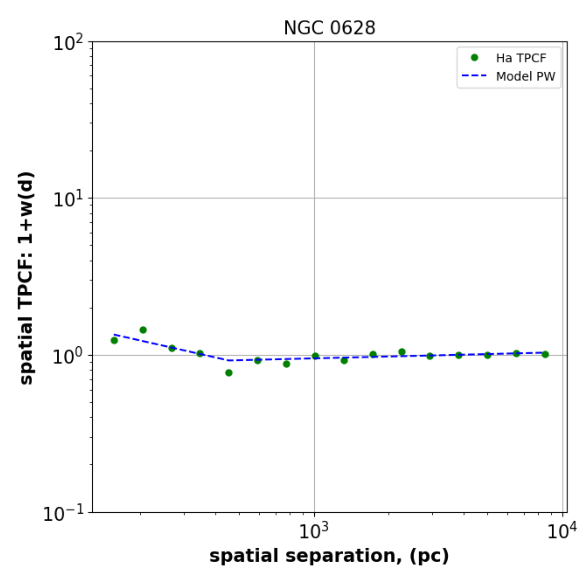
\includegraphics[scale = 0.21]{tpcf_without_cut.png}
            \caption{Without the cut}
            \label{fig:tpcf_without_cut}
        \end{subfigure}
        ~
        \begin{subfigure}{0.45\textwidth}
            \centering
            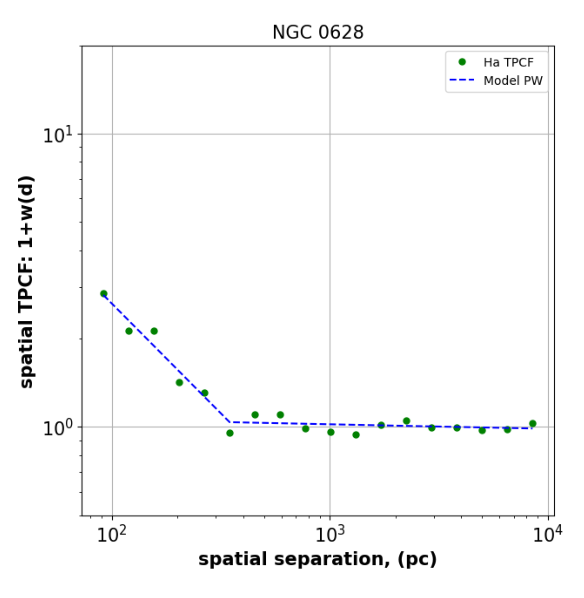
\includegraphics[scale = 0.21]{tpcf_with_cut.png}
            \caption{With the cut}
            \label{fig:tpcf_with_cut}
        \end{subfigure}
    \end{figure}

    \textit{The aim of my project was to understand the physical significance of these thresholds and study the effectiveness of different age estimators of HII regions.}
\end{frame}

\begin{frame}[standout]
    Let's understand a few terms before we proceed:    
\end{frame}

\begin{frame}
    \frametitle{Hierarchical Star Formation}

    Hierarchical star formation is a process where stars are formed in star clusters which exhibit a hierarchical nature of arrangment. This means that stars are formed in small and dense groups which are a part of larger and less dense groups. They look very similar to a geomentric fractal. 

    \begin{figure}[H]
        \centering
        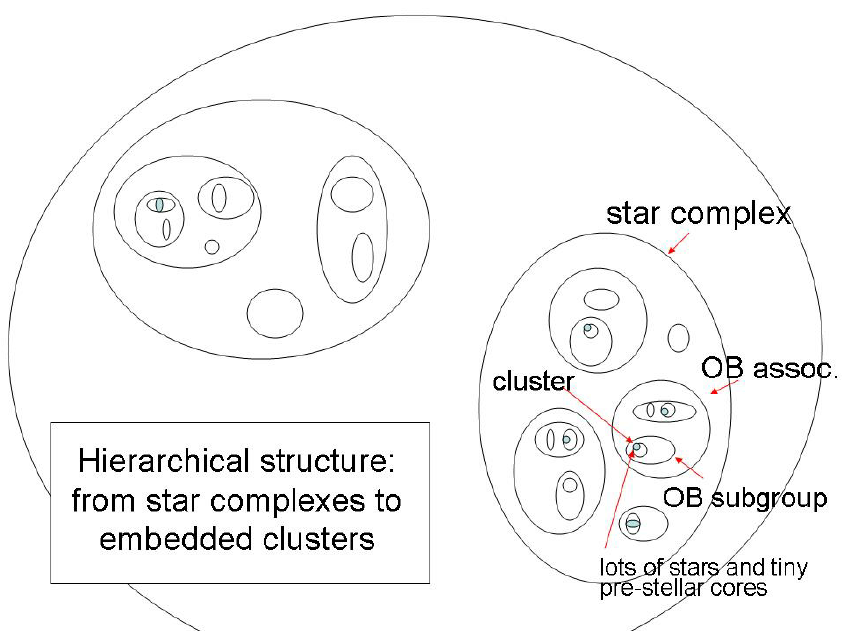
\includegraphics[scale = 0.27]{hierarchy_stars.png}
        \caption{An example of hierarchical star formation \textit{(Elmegreen 2014)}}
        \label{fig:hierarchy_stars}
    \end{figure}
    
\end{frame}

\begin{frame}
    \frametitle{HII regions and $H\alpha$ emissions}

    HII regions are regions of ionized gas around hot, young stars. They are formed when the UV radiation from the OB stars ionizes the surrounding hydrogen gas and causes it to emit $H\alpha$ radiation. 
    \\~\\
    This radiation that is emitted is the source of $H\alpha$ emission lines and it is a strong indicator of star formation.
\end{frame}

\begin{frame}
    \frametitle{Ionization parameter}

    The ionization parameter is a measure of the ionization state of the gas in the HII region. It is defined as the ratio of the incident flux of ionizing photons to the number density of hydrogen atoms. 
    \\~\\
    It is given by: 
    \begin{equation}
        U = \frac{Q}{4\pi R^2 n_H c}
    \end{equation}
    where $Q$ is the rate of ionizing photons at distance $R$, $n_H$ is the number density of hydrogen atoms and $c$ is the speed of light.
\end{frame}

\begin{frame}{Equivalent Width of a spectral line}
    
    The equivalent width of a spectral line is a measure of the strength of the line. It is defined as the width of a rectangle with the same area as the line. 
    \\~\\
    It is given by: 
    \begin{equation}
        EW = \int \left(1 - \frac{F(\lambda)}{F_c(\lambda)}\right) d\lambda
    \end{equation}
    where $F(\lambda)$ is the flux of the line and $F_c(\lambda)$ is the continuum flux.

    \begin{figure}[H]
        \centering
        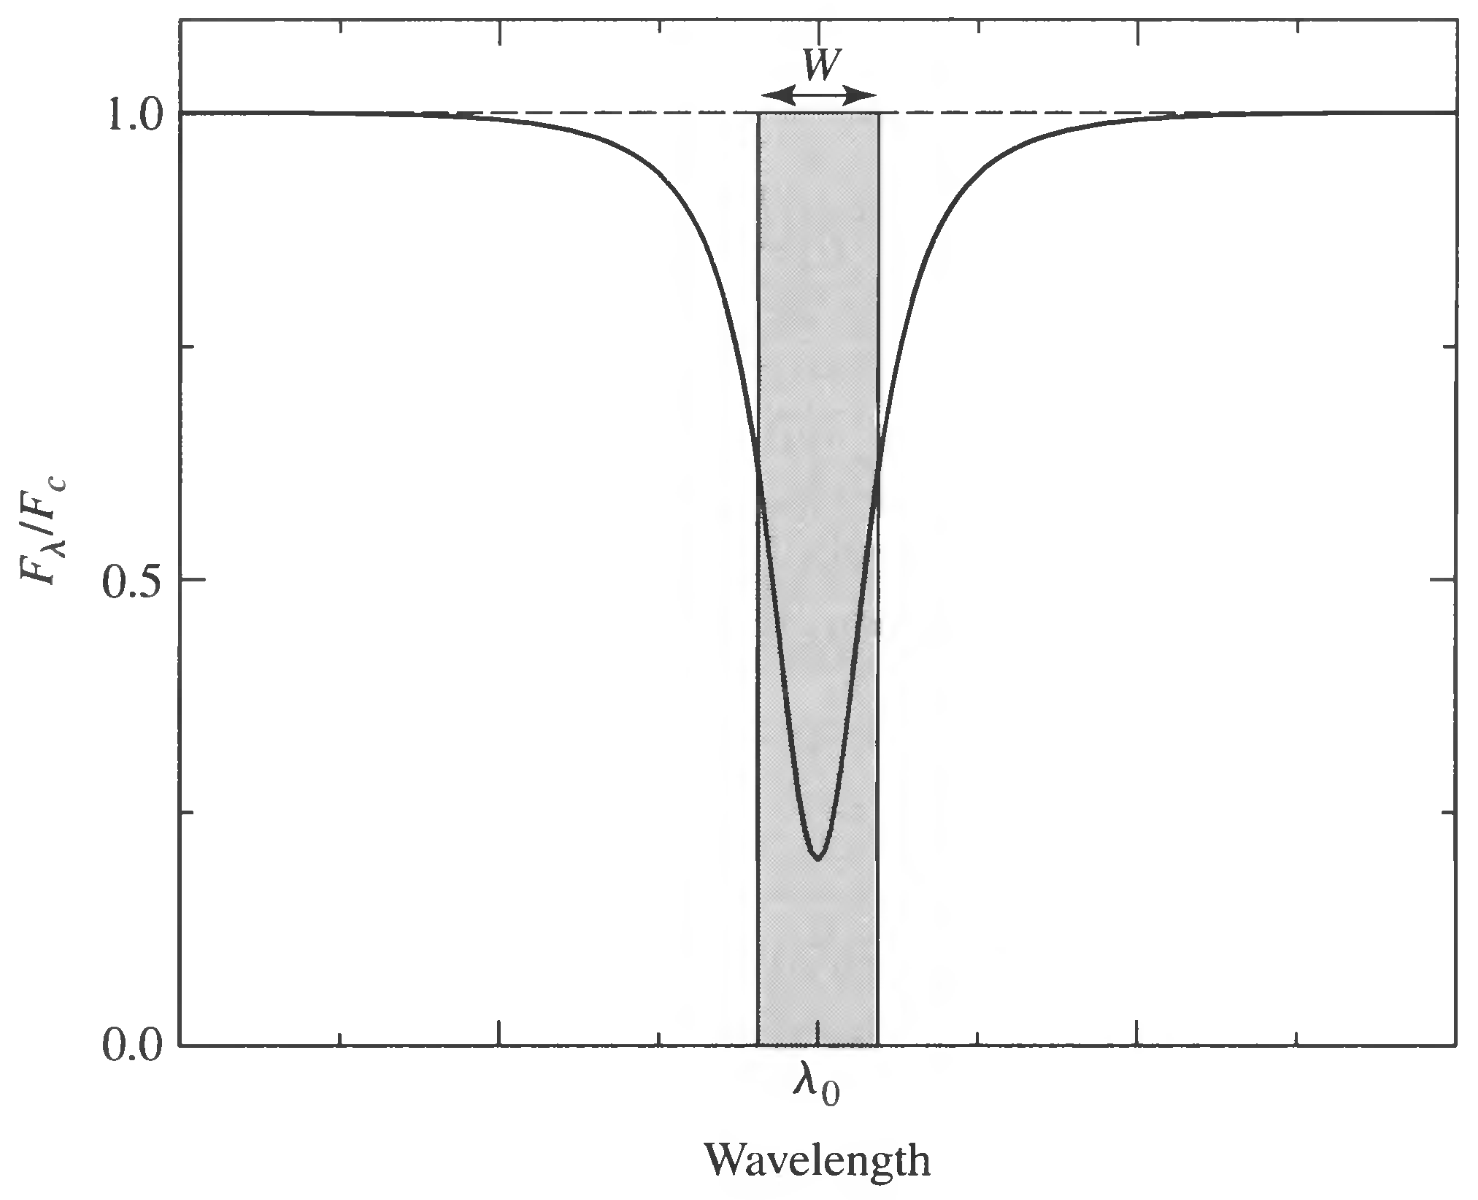
\includegraphics[scale = 0.09]{image3.png}
        \caption{$W$ is the equivalent width of the line (\textit{Carroll and Ostlie 2007})}
        \label{fig:image3}
    \end{figure}

\end{frame}

\begin{frame}
    \frametitle{Flux and Luminosity}

    The flux of a source is the amount of energy emitted per unit area per unit time. It is given by:

    \begin{equation}
        F = \frac{L}{4\pi d^2}
    \end{equation}

    where $L$ is the luminosity of the source and $d$ is the distance of the source from the observer.

    \textit{The luminosity of a source is the total amount of energy emitted per unit time.}
\end{frame}

\begin{frame}
    \frametitle{Spectral Energy Distribution (SED) and Extinction}

    \textbf{SED} is the distribution of energy emitted by a source as a function of wavelength. It is a flux vs wavelength plot of the source.

    \textbf{Extinction} is the process by which the light from a source is absorbed by the dust in the interstellar medium and is re-emitted at longer wavelengths. This causes a loss of flux in at lower wavelengths and an increase in flux at higher wavelengths.
    \\~\\
    A common method to estimate ages of stellar associations is to fit the SED of the region with a model SED. This is known as the \textbf{SED fitting method}.

\end{frame}

\begin{frame}
    \begin{figure}[H]
        \centering
        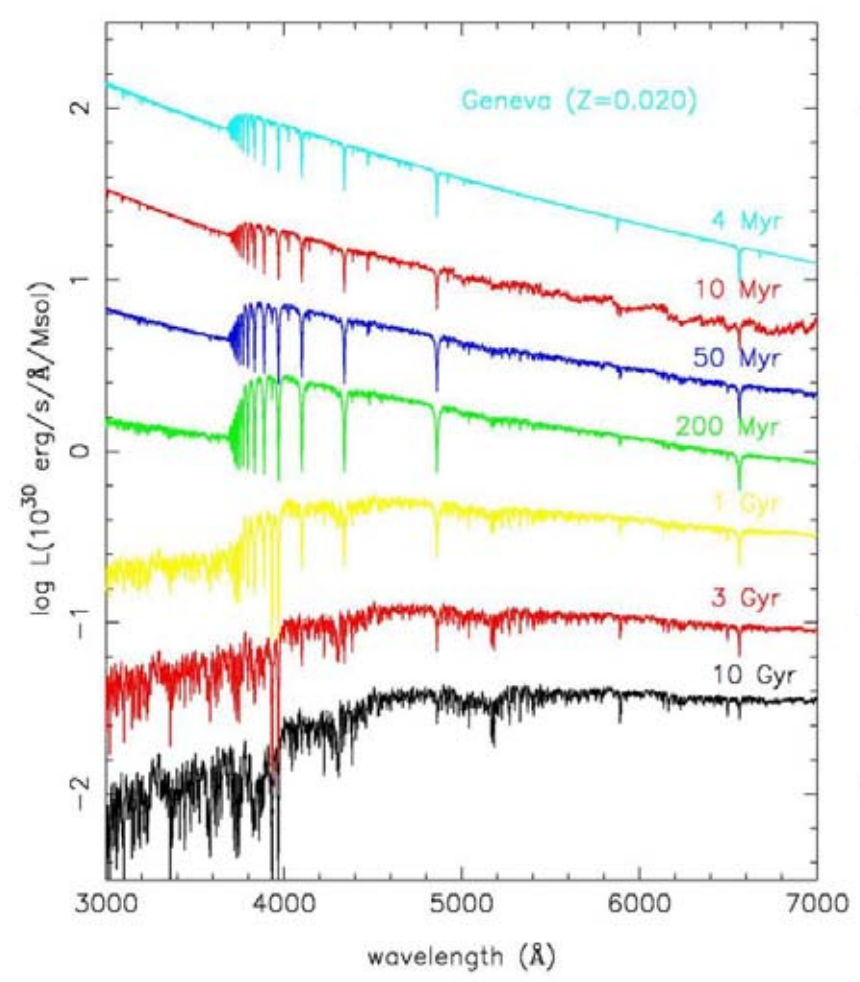
\includegraphics[scale = 0.3]{image21.png}
        \caption{Theoretical Spectral Energy Distribution of a single stellar population (\textit{Image credits: Shashank})}
        \label{fig:image21}
    \end{figure}
    
\end{frame}

\section{Analysis}

\begin{frame}{Age Estimators of HII regions}
    There are different properties of a HII region that can be potentially used as age estimators. Some of them are:

    \begin{itemize}
        \item Equivalent Width of $H\alpha$ line
        \item $H\alpha$ luminosity
        \item Ionization parameter
    \end{itemize}

    My first task was to study the correlation of these properties amongst themselves. 
    This analysis was done using the data from the PHANGS-MUSE HII region catalog $^1$ and the PHANGS Nebular Catalog $^2$ which contains the properties of the HII regions. 

    While a positive correlation between these properties is expected, the obtained correlations differed. 
    
\end{frame}



\begin{frame}{$H\alpha$ luminosity vs Ionization Parameter}
    \begin{figure}
        \centering
        \begin{subfigure}{0.45\textwidth}
            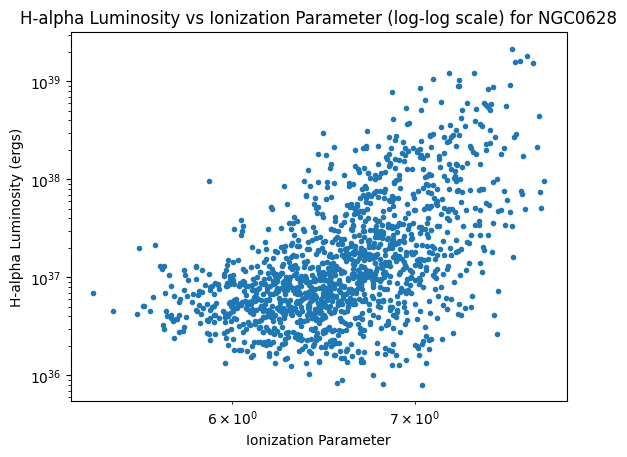
\includegraphics[scale = 0.25]{image5.png}
            \caption{NGC0628}
        \end{subfigure}
        ~
        \begin{subfigure}{0.45\textwidth}
                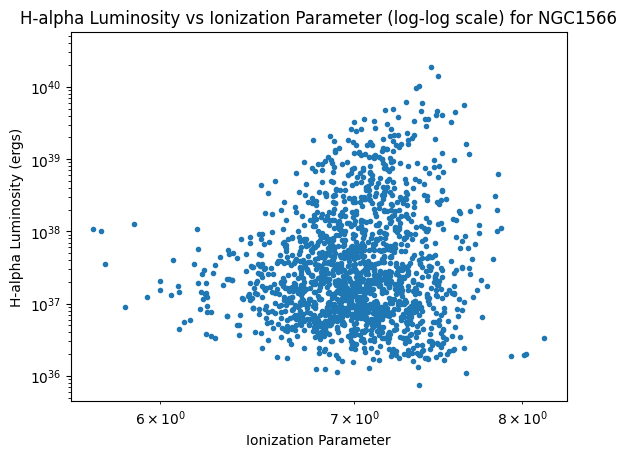
\includegraphics[scale = 0.25]{image6.png}
                \caption{NGC1566}
                \label{fig:image6}
        \end{subfigure}
    \end{figure}

    \begin{figure}[H]
        \centering
        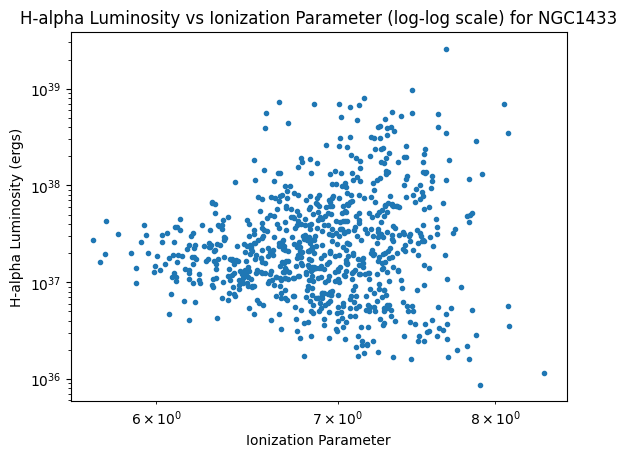
\includegraphics[scale = 0.25]{image7.png}
        \caption*{\textbf{(c)} NGC1433}
        \label{fig:image7}
    \end{figure}
\end{frame}

\begin{frame}{$H\alpha$ equivalent width vs Ionization Parameter}
    \begin{figure}
        \centering
        \begin{subfigure}{0.45\textwidth}
            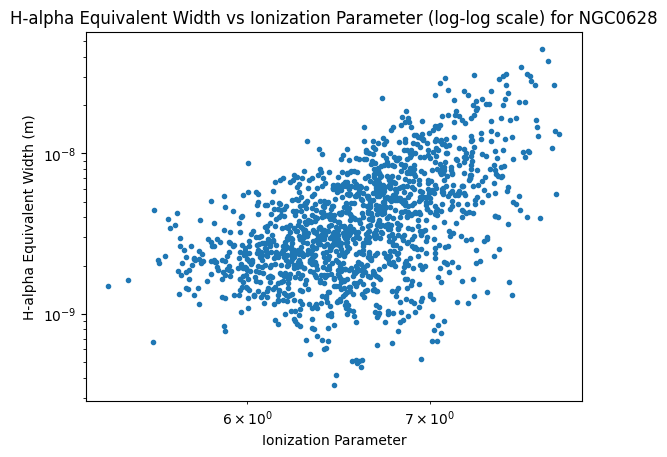
\includegraphics[scale = 0.25]{image35.png}
            \caption{NGC0628}
        \end{subfigure}
        ~
        \begin{subfigure}{0.45\textwidth}
                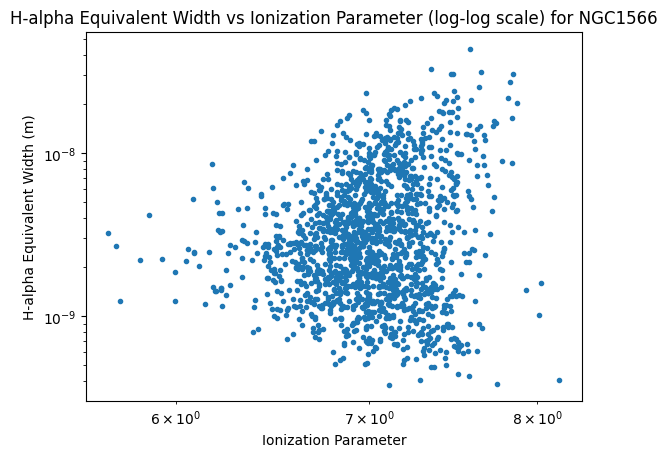
\includegraphics[scale = 0.25]{image33.png}
                \caption{NGC1566}
                \label{fig:image6}
        \end{subfigure}
    \end{figure}

    \begin{figure}[H]
        \centering
        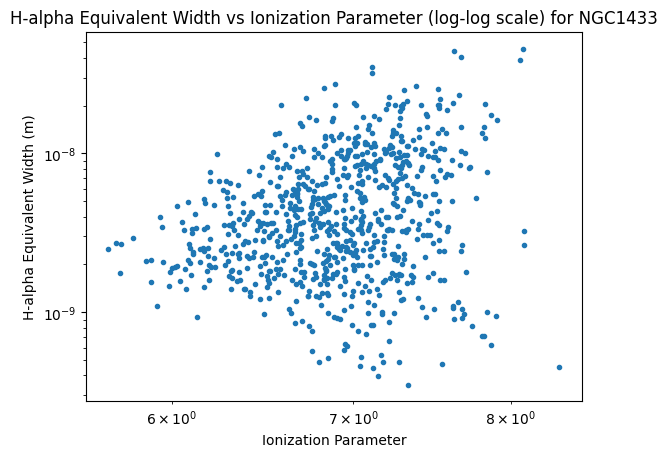
\includegraphics[scale = 0.25]{image31.png}
        \caption*{\textbf{(c)} NGC1433}
        \label{fig:image7}
    \end{figure}
\end{frame}


\begin{frame}{$H\alpha$ equivalent width vs $H\alpha$ Luminosity}
    \begin{figure}
        \centering
        \begin{subfigure}{0.45\textwidth}
            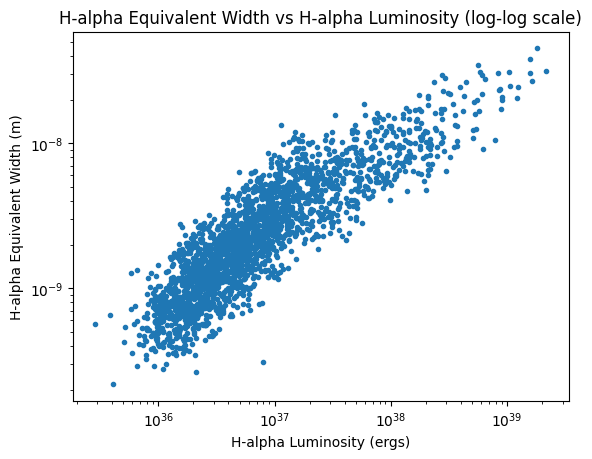
\includegraphics[scale = 0.25]{image36.png}
            \caption{NGC0628}
        \end{subfigure}
        ~
        \begin{subfigure}{0.45\textwidth}
                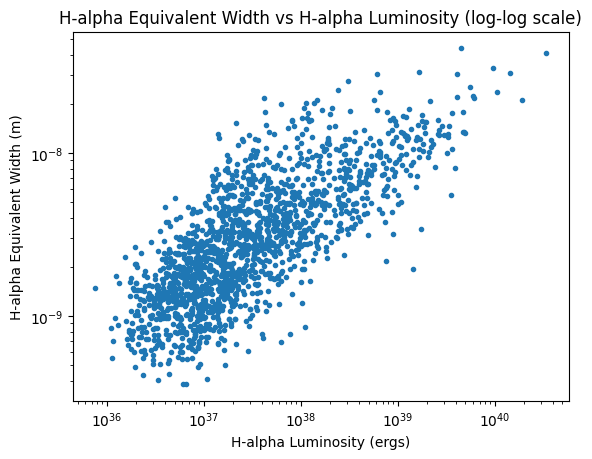
\includegraphics[scale = 0.25]{image34.png}
                \caption{NGC1566}
                \label{fig:image6}
        \end{subfigure}
    \end{figure}

    \begin{figure}[H]
        \centering
        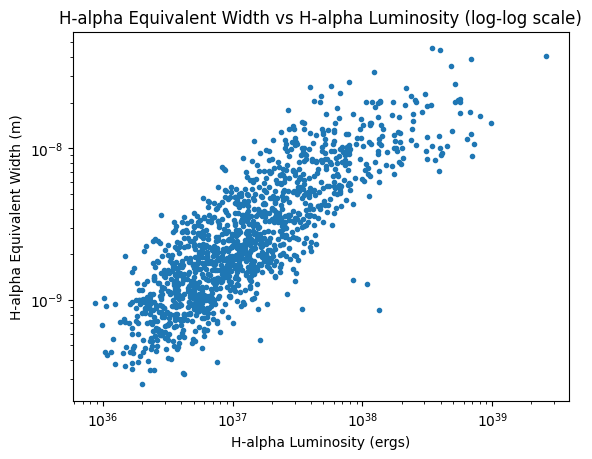
\includegraphics[scale = 0.25]{image32.png}
        \caption*{\textbf{(c)} NGC1433}
        \label{fig:image7}
    \end{figure}
\end{frame}



\begin{frame}{Age Estimators of HII regions}
    The correlation between the properties was not consistent for all the galaxies. 
    \\~\\
    However, when a luminosity cut of $10^{37}$ ergs/sec for the $H\alpha$ luminosity and $6.5$ for the ionization parameter was applied, a somewhat linear correlation was observed. 
    \\~\\
    This is consistent with Nimya's findings.
\end{frame}

\begin{frame}{Correlation between parameters for all galaxies}
    \begin{figure}
        \centering
        \begin{subfigure}{0.45\textwidth}
            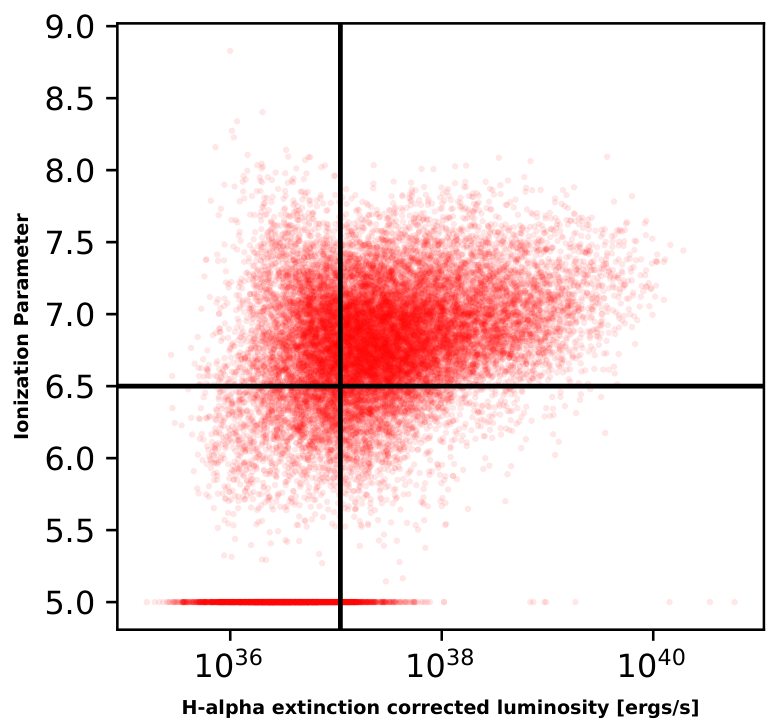
\includegraphics[scale = 0.15]{image37.png}
            \caption{luminosity vs ion. param}
        \end{subfigure}
        ~
        \begin{subfigure}{0.45\textwidth}
                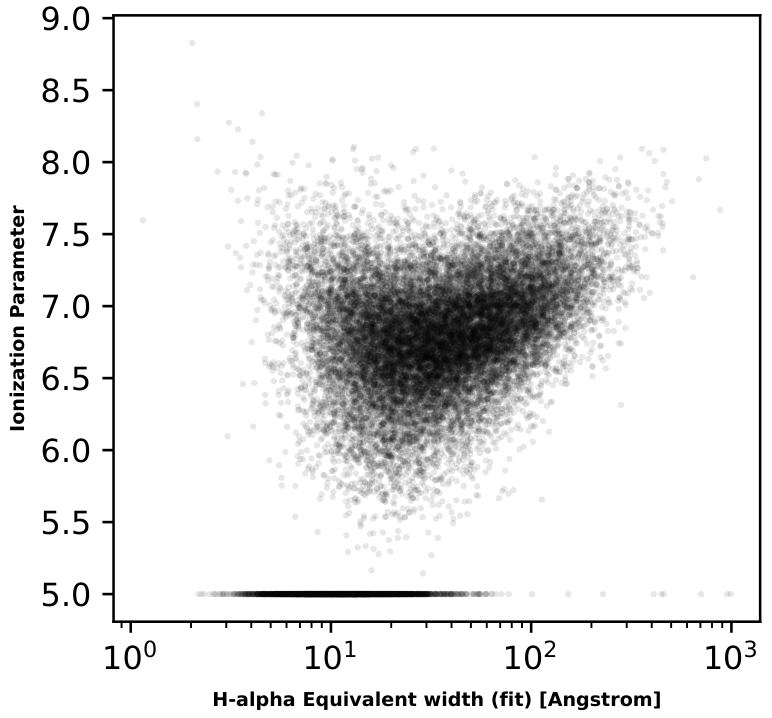
\includegraphics[scale = 0.15]{image38.png}
                \caption{Eq width vs ion. param}
                \label{fig:image6}
        \end{subfigure}
    \end{figure}

    \begin{figure}[H]
        \centering
        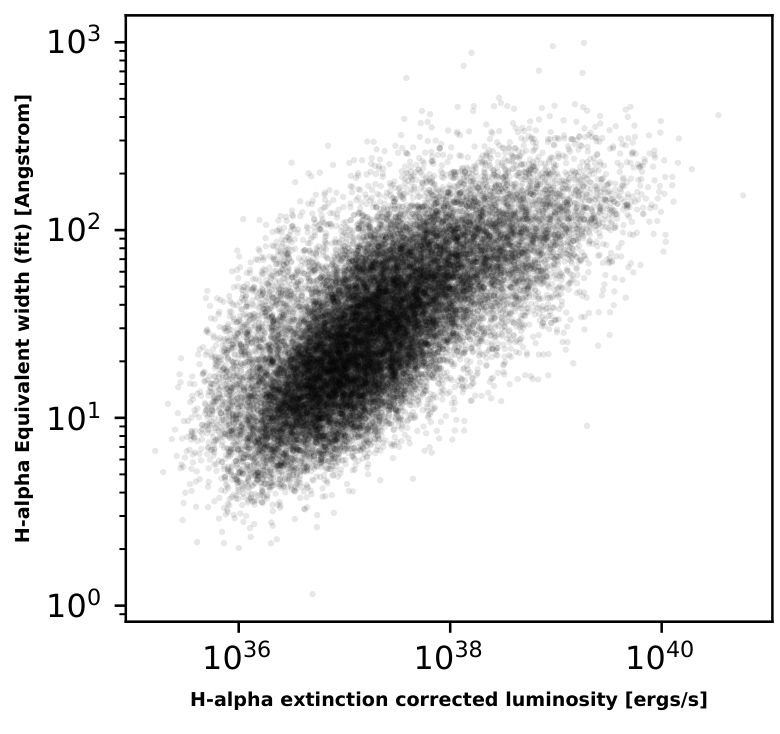
\includegraphics[scale = 0.15]{image39.png}
        \caption*{\textbf{(c)} Eq. width vs luminosity}
        \label{fig:image7}
    \end{figure}
    
\end{frame}



\begin{frame}{Age Estimators of HII regions}
    A similar analysis was done by F. Scheuermann et al. 2023 $^3$ where they studied the HII regions obtained from the PHANGS-MUSE survey and corresponding stellar associations as through the PHANGS-HST survey. 
    \\~\\
    They found that the age estimators were more consistently correlated with each other as well as the age of the stellar associations. These ages were obtained using the SED fitting method. 

    It is to be noted that the paper suggests the fainter unmatched HII regions with luminosity $ < 10^{37}$ ergs/sec could be ionized by a single O-type star or a very small star cluster. 
\end{frame}

\begin{frame}
\begin{figure}[H]
    \centering
    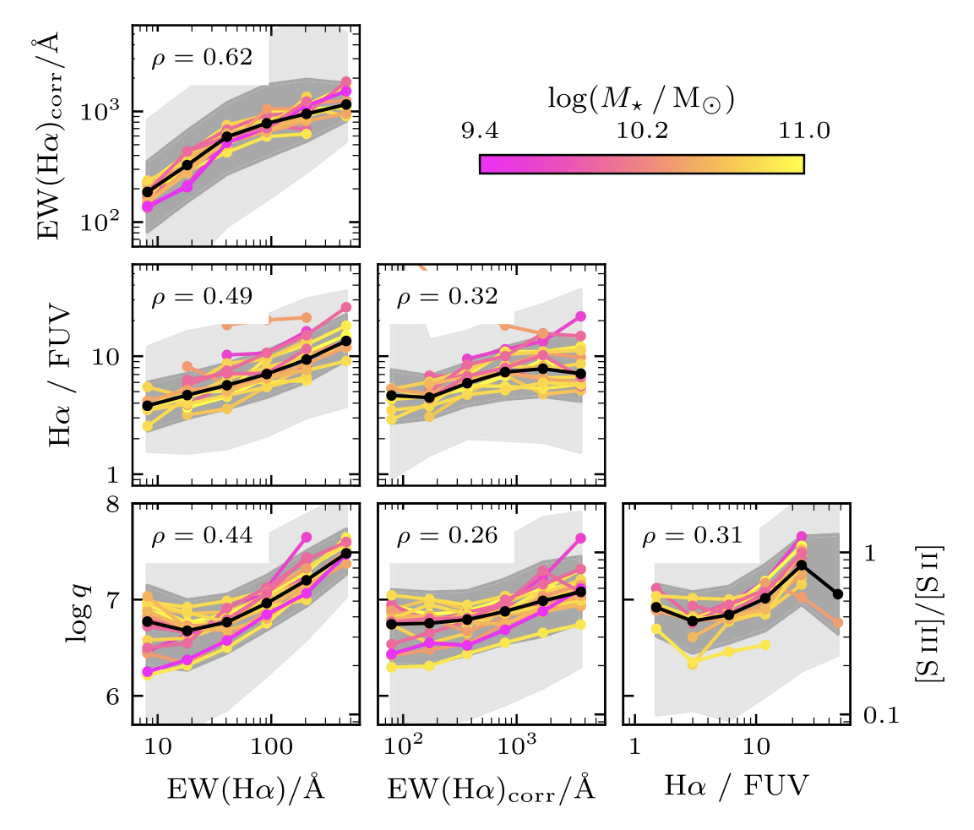
\includegraphics[scale = 0.3]{image8.png}
    \caption{Observed correlation between the age estimators (\textit{Scheuermann et al. 2023})}
    \label{fig:image8}
\end{figure}

\end{frame}

\begin{frame}
    \begin{figure}[H]
        \centering
        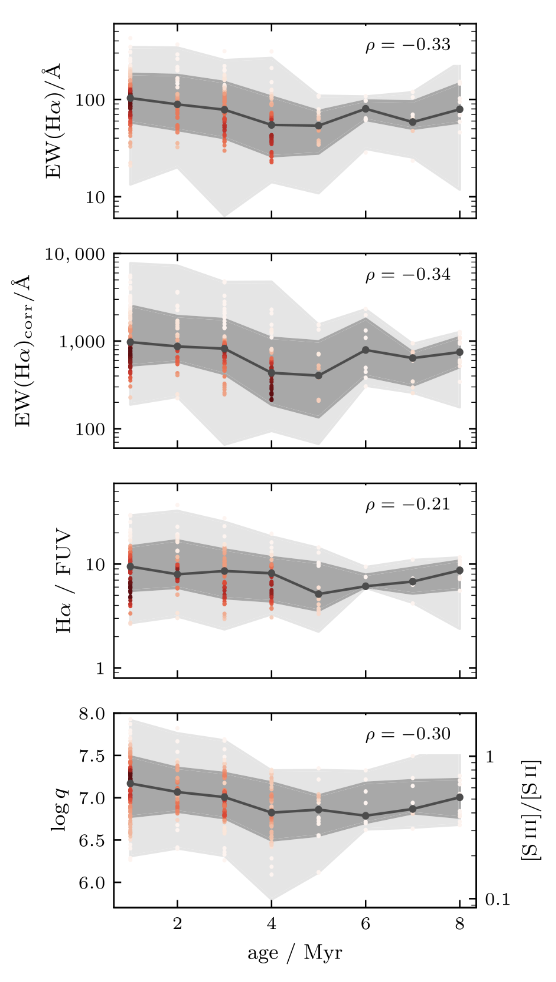
\includegraphics[scale = 0.3]{image10.png}
        \caption{Correlation between the age estimators and the age of the stellar associations (\textit{Scheuermann et al. 2023})}
        \label{fig:image10}
    \end{figure}
    
\end{frame}

\begin{frame}{Age Estimators of HII regions}
    From the above plots, we see that all the age estimators decrease with the age of the stellar associations. However, this is observed only up until the 6 Myr mark. After this, the age estimators remain constant or increase, which is against the expected trend. 

    The paper concludes its analysis within the 8 Myr mark, but on extending the analysis to observe if the same increasing trend continues, the following was observed: 

    \begin{figure}
        \centering
        \begin{subfigure}{0.45\textwidth}
            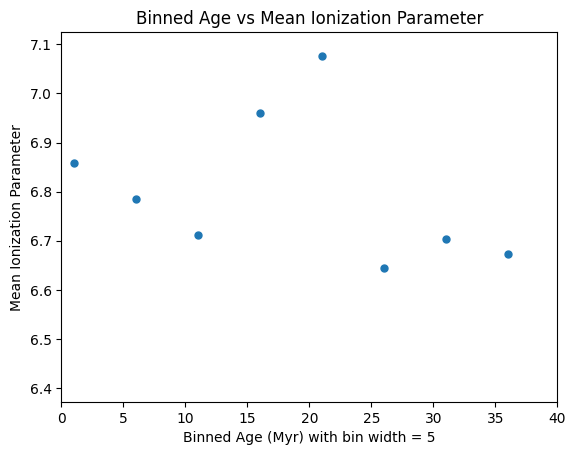
\includegraphics[scale = 0.3]{image22.png}
            %\caption{}
            \label{fig:image19}
        \end{subfigure}
        ~
        \begin{subfigure}{0.45\textwidth}
            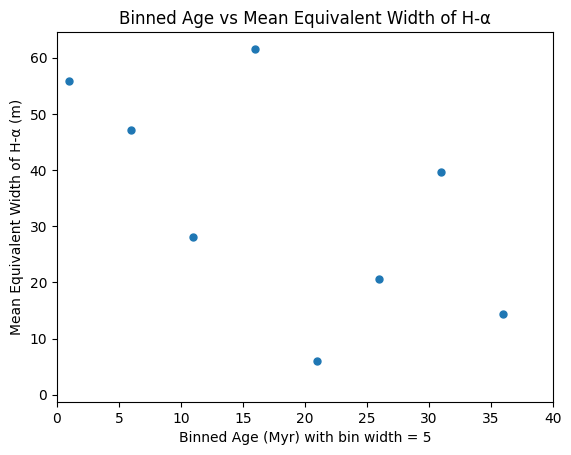
\includegraphics[scale = 0.3]{image23.png}
            %\caption{}
            \label{fig:image20}
        \end{subfigure}
        
    \end{figure}
\end{frame}

\begin{frame}{Age Estimators of HII regions}
    Another important point to note here that the extinction was calculated using the SED fitting as well as the Balmer decrement method. 

    A comparison of the extinction obtained from the two methods was also done: 

    \begin{figure}[H]
        \centering
        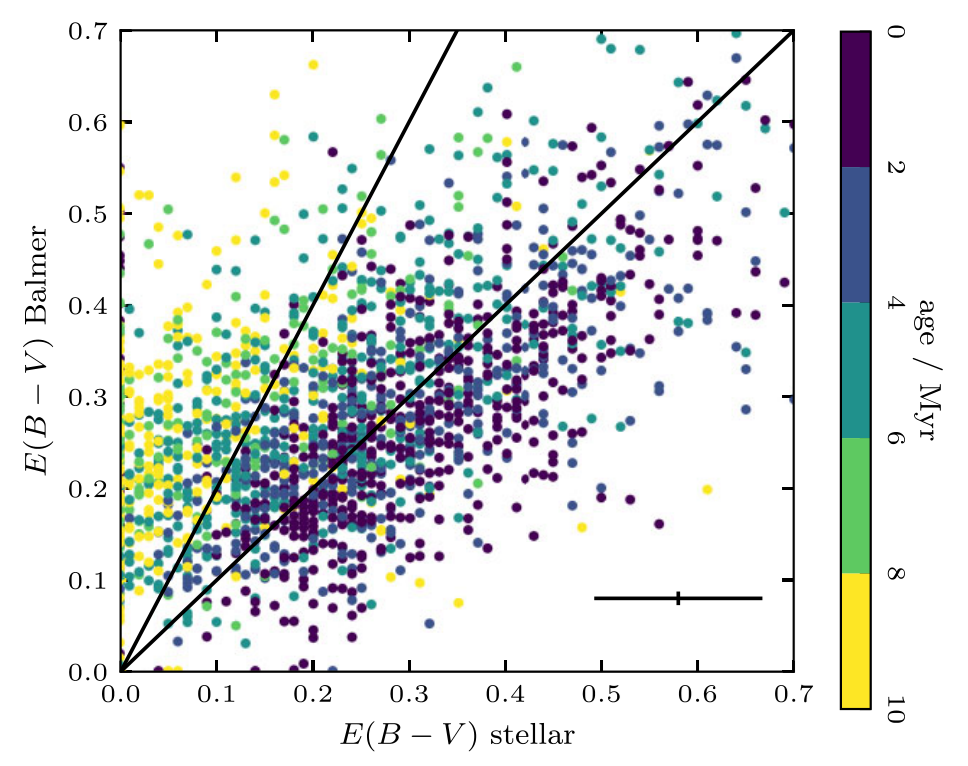
\includegraphics[scale = 0.19]{image29.png}
        \caption{Comparison of the extinction obtained from the two methods (\textit{Scheuermann et al. 2023})}
        \label{fig:image29}
    \end{figure}
    
            
    
\end{frame}

\begin{frame}{Age Estimators of HII regions}
    We observe that for younger regions, the extinction obtained through both methods is consistent. However, for older regions, the extinction obtained through the SED fitting method is lower. 

    This could occur due to an error in the SED fit where it identifies younger but more extincted regions as older and less extincted. 

    
\end{frame}

\begin{frame}{Analysis using UVIT data}
    To overcome this, we tried to perform a similar analysis using the PHANGS-MUSE and AstroSat's UVIT data for the galaxy NGC1566. Shashank had analyzed the UVIT data and used StarBurst99 to obtain the ages of the stellar associations. 
    \\~\\
    The two catalogues were cross matched using TOPCAT and the ages of were compared to the different age estimators. 

    But again, we dont see a consistent correlation between the age estimators and the age of the stellar associations.
\end{frame}

\begin{frame}
    \begin{figure}
        \centering
        \begin{subfigure}{0.45\textwidth}
            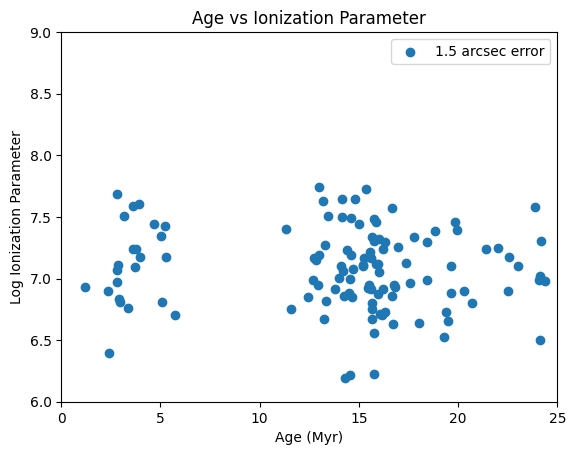
\includegraphics[scale = 0.3]{image24.png}
            \caption{Ionization Parameter vs age}
        \end{subfigure}
        ~
        \begin{subfigure}{0.45\textwidth}
            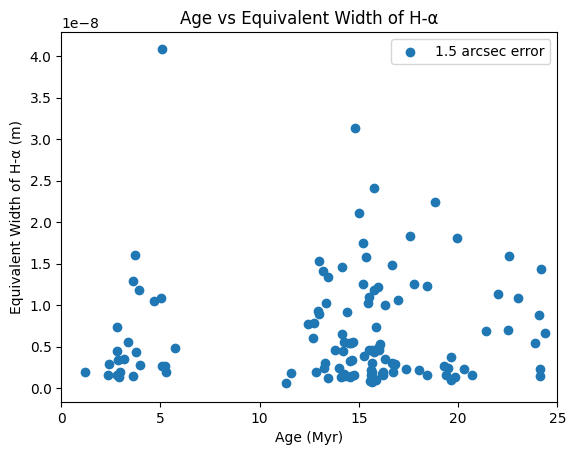
\includegraphics[scale = 0.3]{image25.png}
            \caption{Equivalent Width vs Age}
        \end{subfigure}
    \end{figure}

    \begin{figure}[H]
        \centering
        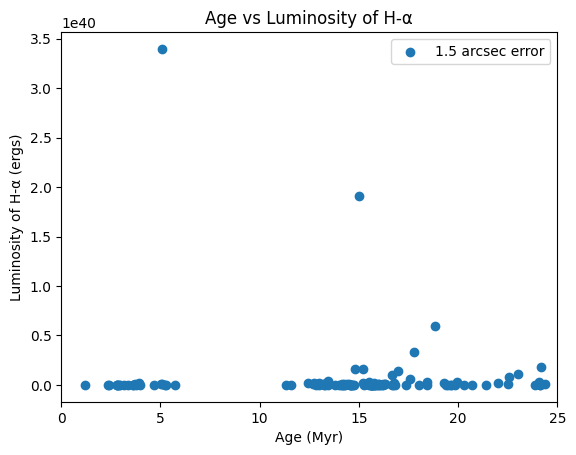
\includegraphics[scale = 0.3]{image26.png}
        \caption*{\textbf{(c)} H$\alpha$ luminosity vs age}
        \label{fig:image17}
    \end{figure}
\end{frame}

\section{Conclusion and Remarks}

% Conclusion
\begin{frame}{Conclusion}
    \begin{itemize}

    \item The analysis of the age estimators of the HII regions showed that the properties of the HII regions are correlated with each other and the age of the stellar associations. However this correlation is not consistent across all galaxies and different data sets. 
    \item If on further analysis the correlation is found to be consistent, the ionization parameter would be a better age estimator and it gives us the advantage of directly determining the age of the HII region without the need for any stellar associations. 
    \item The thresholds set by Nimya for the $H\alpha$ luminosity and the ionization parameter enable us to observe only the most recent star formation events, which are expected and observed to show a hierarchical nature.
    
    \end{itemize}
\end{frame}

% Future Work
\begin{frame}{Future Work}
    \begin{itemize}
        \item More detailed analysis of the UVIT data and the PHANGS-MUSE data is needed. 
        \item The physical significance of the thresholds set by Nimya needs to be understood, especially the luminosity cut which could be related to a single O-type star or a small star cluster, as suggested by F. Scheuermann et al. 2023.
    
    \end{itemize}
\end{frame}

% Learning Outcomes 
\begin{frame}{My Learning Outcomes}
    Through this project, I learnt the following:
    \begin{itemize}
        \item The theory of star formation and the properties of HII regions.
        \item Using different catalogues and tools like TOPCAT to cross match data and perform analysis on them. 
        \item The basics of SED fitting and UVIT data reduction and analysis. 
        \item Using StarBurst99 to obtain the ages of stellar associations and HII regions.
    \end{itemize}
\end{frame}

% Acknowledgements
\begin{frame}{Acknowledgements}
    I would like to thank Prof. Smitha Subramanian for giving me the opportunity and her guidance throughout the project. I also really appreciate the freedom she gave me to explore different aspects of the project. 

    I would also like to express my sincere gratitude to Shashank for his help in making me understand a lot of concepts and for his guidance in the analysis throughout the project.

    Last but not the least, I would like to thank the institute for providing me with the opportunity to work on this project and my parents and friends for their constant support.
\end{frame}

\begin{frame}{References}
    \begin{enumerate}
        \item ``PHANGS–MUSE: The H II region luminosity function of local star-forming galaxies'' by Santoro et al. 2021, 	https://doi.org/10.1051/0004-6361/202141907
        \item B Groves et al. 2023, The PHANGS–MUSE nebular catalogue, Monthly Notices of the Royal Astronomical Society, Volume 520, Issue 4, April 2023, Pages 4902–4952, https://doi.org/10.1093/mnras/stad114
        \item ``Stellar associations powering H II regions – I. Defining an evolutionary
        sequence'' by F. Scheuermann et al. 2023, https://doi.org/10.1093/mnras/stad878
        \item ``Tracing young star-forming clumps in the nearby flocculent spiral galaxy NGC 7793 with UVIT imaging'' by Mondal et al. (2021)
    \end{enumerate}
    
\end{frame}



\end{document}